
\section{Motivation}

Knowing your machine is a major advantage when trying to optimize high-performance scientific code. \iaca\ (Intel Architecture Code Analyzer) \cite{iaca} is a tool by Intel to analyze \emph{x86} machine code with respect to a specific microarchitecture. However, it has some drawbacks that oftentimes prevent it from being useful in practice, mainly because it doesn't support the most recent processors. \iaca\ $3.0$, which was released in late 2017, supports the \nth{4} (Haswell) to the \nth{6} (Skylake) generation of Intel core microarchitectures. Skylake was released in 2015. \iaca\ $2.3$ additionally supports the \nth{2} (Sandy Bridge) and the \nth{3} (Ivy Bridge) generation. So at the time of writing \iaca\ is about three years behind and its further development remains unclear.\\
The second complication is that \iaca\ is closed source. Its user guide \cite{userguide} is the only documentation it has which provides little to no information about how it actually computes its output. As a result a user will often find himself wondering how its output fits the analyzed program.\\
In this work we present \suaca\ (Saarland University Architecture Code Analyzer), an open source alternative. It uses measurements provided by \cite{Andreas} which are parsed during runtime. This way a user does not rely on a software update of the tool as he can simply perform the measurements on his own, should we not already support his microarchitecture. At the time of writing \suaca\ supports all Intel core microarchitectures from the \nth{1} (Nehalem) to the \nth{8} (Coffee Lake) generation, except for the server variant of Skylake.
\newpage

\section{Intel's Microarchitectures}


In order to understand some the computations described in the following sections, we give a brief overview over Intel's microarchitectures. They use the \emph{x86} instruction set. However, a single \emph{x86} instruction will be not executed

% Define the layers to draw the diagram
\pgfdeclarelayer{background}
\pgfdeclarelayer{background1}
\pgfdeclarelayer{foreground}
\pgfsetlayers{background,background1,main,foreground}

% Define block styles
\tikzstyle{nodeStyle} = [draw, text width=6cm,  minimum height=1.75em, text centered]
\tikzstyle{port} = [draw, fill={rgb,255:red,135; green,220; blue,170}, text width=0.75cm, font=\fontsize{6}{7.2}\sffamily, text centered]
\tikzstyle{FU} = [draw, fill={rgb,255:red,212; green,170; blue,0}, text width=5.0em, font=\fontsize{6}{7.2}\sffamily, rotate=90, text centered]
\tikzstyle{arrow} = [draw, thick, color=black!80, font=\footnotesize\sffamily]

% Draw background
\newcommand{\background}[7]{%
    \begin{pgfonlayer}{background}
        % Left-top corner of the background rectangle
        \path (#1.west |- #2.north)+(-1,0.4) node (a1) {};
        % Right-bottom corner of the background rectangle
        \path (#3.east |- #4.south)+(+0.4,#5) node (a2) {};
        % Draw the background
        \path[fill=#6, draw=black!50]
        (a1) rectangle (a2);
        \path let \p{x}=(a1), \p{y}=($(a1)!0.5!(a2)$) in (\x{x}, \y{y})+(0.5,0) node (u1)[rotate=90]
        {#7};
\end{pgfonlayer}}

\begin{figure}
    \centering
    \resizebox{!}{0.8\textheight}{
    \begin{tikzpicture}[scale=0.8,transform shape,font=\fontsize{11}{13.2}\sffamily]
    % Draw diagram elements
    \path node (nIC) [nodeStyle, fill={rgb,255:red,249; green,177; blue,166}] {Instruction Cache};
    \path (nIC.south)+(0.0,-1.0) node (nFD) [nodeStyle, fill={rgb,255:red,171; green,204; blue,227}] {Instruction Fetch \& Decode};
    \path (nFD.south)+(0.0,-1.3) node (nReorder) [nodeStyle, fill={rgb,255:red,198; green,233; blue,175}] {Reorder Buffer};
    \path (nReorder.south)+(0.0,-1.0) node (nRS) [nodeStyle, fill={rgb,255:red,135; green,220; blue,170}] {Scheduler};
    \path (nRS.south)+(-2.5,0.0) node[anchor=north] (nPort0) [port] {Port 0};
    \path (nRS.south)+(-1.5,0.0) node[anchor=north] (nPort1) [port] {Port 1};
    \path (nRS.south)+(-0.5,0.0) node[anchor=north] (nPort2) [port] {Port 2};
    \path (nRS.south)+(0.5,0.0) node[anchor=north] (nPort3) [port] {Port 3};
    \path (nRS.south)+(1.5,0.0) node[anchor=north] (nPort4) [port] {Port 4};
    \path (nRS.south)+(2.5,0.0) node[anchor=north] (nPort5) [port] {Port 5};
    
    \path (nPort0.south)+(0,-0.75) node[anchor=east] (nPort0FU) [FU] {ALU, V-MUL, \dots};
    \path (nPort1.south)+(0,-0.75) node[anchor=east] (nPort1FU) [FU] {ALU, V-ADD, \dots};
    \path (nPort2.south)+(0,-0.75) node[anchor=east] (nPort2FU) [FU] {Load, AGU};
    \path (nPort3.south)+(0,-0.75) node[anchor=east] (nPort3FU) [FU] {Load, AGU};
    \path (nPort4.south)+(0,-0.75) node[anchor=east] (nPort4FU) [FU] {Store Data};
    \path (nPort5.south)+(0,-0.75) node[anchor=east] (nPort5FU) [FU] {ALU, JMP, \dots};
    
    \begin{pgfonlayer}{background1}
    \path (nPort0FU.north |- nPort0FU.east)+(-0.25,0.25) node (ee_tl) {};
    \path (nPort5FU.south |- nPort5FU.west)+(+0.25,-0.25) node (ee_br) {};
    \path[fill={rgb,255:red,95; green,211; blue,188}, draw=black!50, rounded corners] (ee_tl) rectangle (ee_br);
    \end{pgfonlayer}
    
    \path let \p{x}=(nRS.south), \p{y}=(ee_br.south) in (\x{x}, \y{y})+(0,-1.0) node (nL1D)
    [nodeStyle, fill={rgb,255:red,249; green,177; blue,166}] {L1 Data Cache};
    \path (nL1D.south)+(0.0,-1.0) node (nL2) [nodeStyle, fill={rgb,255:red,249; green,177; blue,166}] {L2 Cache};
    
    % Draw arrows between elements
    \draw [->, arrow] (nIC.south) -- (nFD.north);
    \draw [->, arrow] (nFD.south) -- node [right] {4--6 \textnormal\microops} +(0,-0.6) -- (nReorder.north);
    \draw [->, arrow] (nReorder.south) -- node [right] {\textnormal\microops} (nRS.north);
    
    \draw [->, arrow, font=\fontsize{6}{7.2}\sffamily] (nPort0.south) -- node [right] {\textnormal\microop} +(-0,-0.5) -- (nPort0FU.east);
    \draw [->, arrow, font=\fontsize{6}{7.2}\sffamily] (nPort1.south) -- node [right] {\textnormal\microop} +(-0,-0.5) -- (nPort1FU.east);
    \draw [->, arrow, font=\fontsize{6}{7.2}\sffamily] (nPort2.south) -- node [right] {\textnormal\microop} +(-0,-0.5) -- (nPort2FU.east);
    \draw [->, arrow, font=\fontsize{6}{7.2}\sffamily] (nPort3.south) -- node [right] {\textnormal\microop} +(-0,-0.5) -- (nPort3FU.east);
    \draw [->, arrow, font=\fontsize{6}{7.2}\sffamily] (nPort4.south) -- node [right] {\textnormal\microop} +(-0,-0.5) -- (nPort4FU.east);
    \draw [->, arrow, font=\fontsize{6}{7.2}\sffamily] (nPort5.south) -- node [right] {\textnormal\microop} +(-0,-0.5) -- (nPort5FU.east);
    
    \draw [<->, arrow] (nPort2FU.west) -- (nPort2FU.west |- nL1D.north);
    \draw [<->, arrow] (nPort3FU.west) -- (nPort3FU.west |- nL1D.north);
    \draw [->, arrow] (nPort4FU.west) -- (nPort4FU.west |- nL1D.north);
    
    \draw [<->, arrow] (nL1D.south) -- (nL2.north);
    \draw [->, arrow] (nL2.east) -- +(+0.8,-0.0) |- (nIC.east);
    
    \background{nIC}{nIC}{nL2}{nFD}{-0.7}{{rgb,255:red,255; green,246; blue,213}}{Front End}
    \background{nReorder}{nReorder}{nL2}{ee_br}{-0.5}{{rgb,255:red,213; green,255; blue,230}}{Execution Engine}
    \background{nL1D}{nL1D}{nL1D}{nL2}{-0.4}{{rgb,255:red,252; green,222; blue,212}}{Memory}
    \end{tikzpicture}}
    \caption{Pipeline of Intel Core CPUs (simplified).}
\end{figure}

on the CPU as it is, but the instruction will be translated into a sequence of so called \microops, which can then be executed. Unfortunately, there is little to no official documentation about those \microops, neither about the functionality of an individual one nor about their interaction with each other. From the measurements we can conclude that each microarchitecture has its own \microops\ which makes it even harder to find reliable information.\\ \autoref{fig:Pipeline} shows a sketch of a microarchitecture by Intel. We can see the front-end including the decoder unit which is responsible for the translation of the instructions into the \microops. In our simulation, we will only consider the number of \microops\ the front-end produces each cycle, which are currently $4$--$6$ depending on the architecture. Our main interest is focused on the execution engine or more precisely on the scheduler (or reservation station) and the ports. The scheduler is responsible for the distribution of the \microops\ over the ports. As mentioned before, a certain amount of those will be loaded into it by the front-end in each cycle. It has a maximum capacity, which also depends on the specific architecture (the scheduler of the Sandy Bridge architecture we will be using for most of our examples has a capacity of $54$). The most important property we can observe from this figure are the ports. Each port can be seen as a pipeline that a \microop\ can run through in order to be executed. The ports themselves hold the actual execution units of the processor like the \emph{ALU}, \emph{MULTIPLEXER} and so on. Every port can hold a single \microop\ per cycle and they support pipelining, which means that the port can be used again by another \microop\ in the next cycle while others are still inside the execution units. The only exception from this is the \emph{DIVIDER} unit which is slow at executing and can be blocked for multiple cycles. Usually it is not necessary that the \microops\ are executed in program order. The so called out-of-order execution is possible whenever there is no dependency between the respective \emph{x86} instructions or the \microops\ themselves.
 
 %\begin{wrapfigure}[25]{l}{0.6\textwidth}
 %   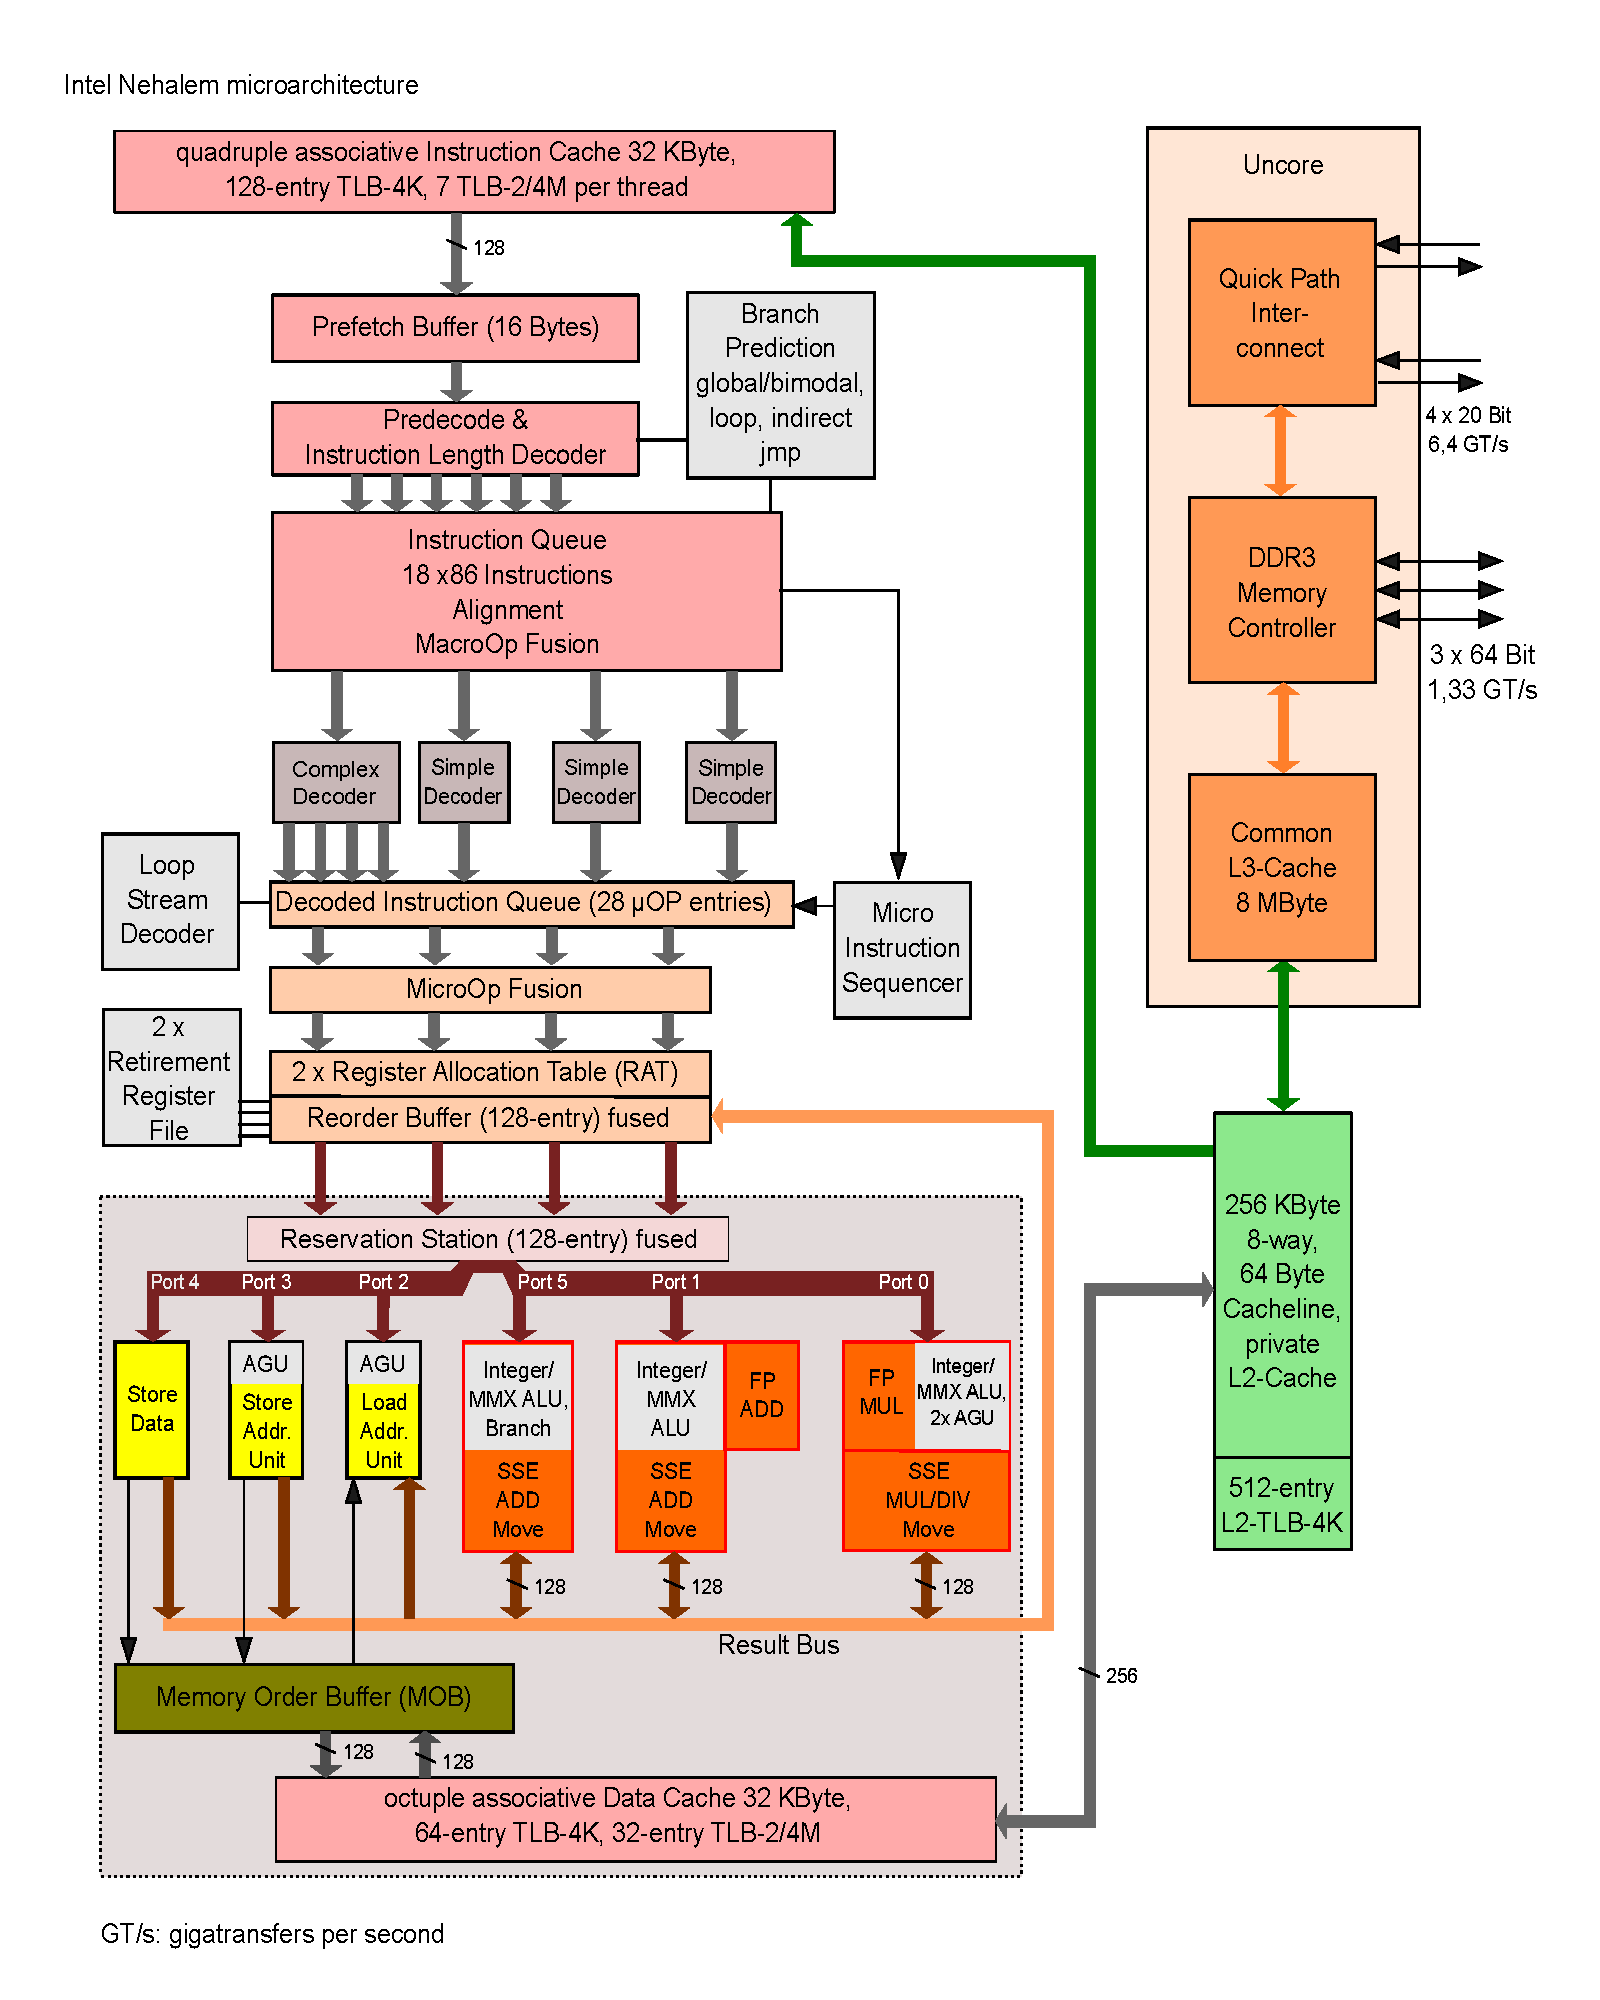
\includegraphics[width=0.6\textwidth]{Intel_Nehalem_arch}
 %  \caption{Intel Nehalem architecture \cite{nehalem}}
 % \label{fig:NHMfull}
 %\end{wrapfigure}
 
 
 %\begin{wrapfigure}[15]{r}{0.6\textwidth}
 %  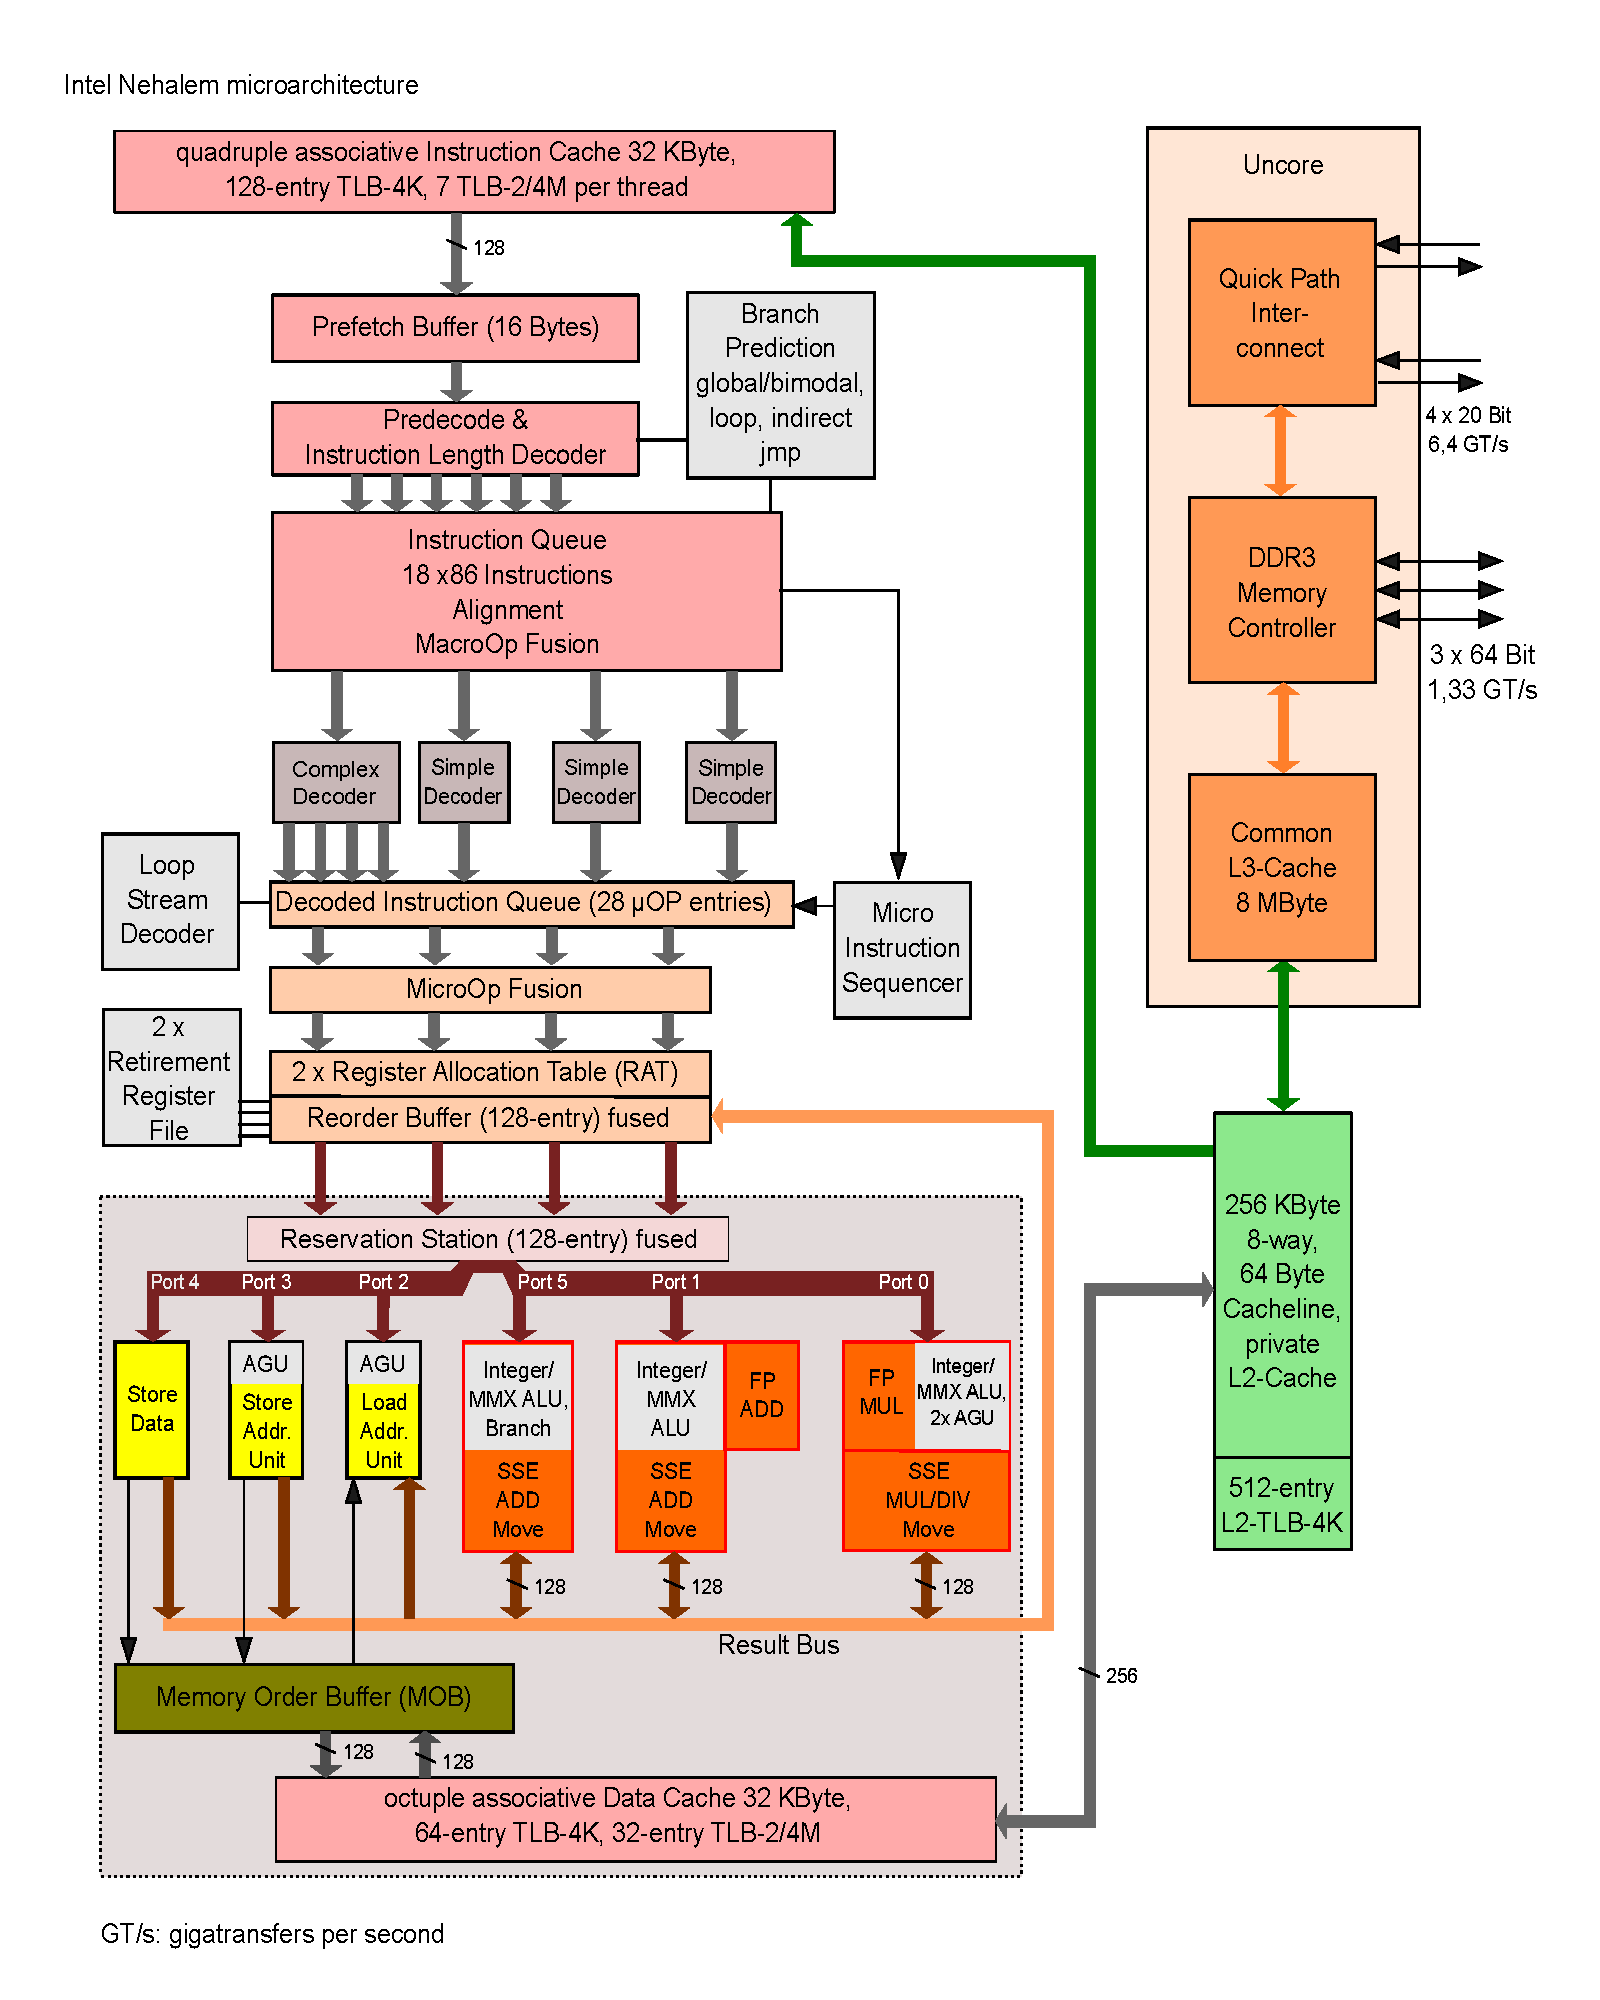
\includegraphics[clip, trim=0.5cm 2cm 9.78cm 20cm,width=0.6\textwidth]{Intel_Nehalem_arch}
 %\caption{Detailed view \cite{nehalem}}
 %\label{fig:NHMdetail}
 %\end{wrapfigure}
 
\section{\iaca's Analysis} 

In order to use \iaca\ one first has to prepare the code with the two markers that are defined in the \emph{iacaMarks.h} header. As \iaca\ is mostly used to analyze innermost loops of scientific code we will show how those markers are inserted there:

\begin{mdframed}[backgroundcolor=light-gray, roundcorner=10pt,leftmargin=1, rightmargin=1, innerleftmargin=15, innertopmargin=1,innerbottommargin=1, outerlinewidth=1, linecolor=light-gray]
    \begin{lstlisting}
    #include "iacaMarks.h"
    
    int main(void) {
    
        while (condition) {
            (*@\textcolor{Green}{IACA\_START}  @*)
            //Some code here
        }
        (*@\textcolor{Green}{IACA\_END}  @*)
    
        return 0;
    }
    \end{lstlisting}
\end{mdframed}

When writing assembly code one can simply insert the markers that are defined in the \emph{iacaMarks.h} header manually.\\
In the following we will perform a throughput analysis with \iaca\ $2.3$. The \emph{throughput} is the average number of cycles needed to execute the body of the loop and is therefore the value a programmer should try to optimize.\\ 
The \emph{latency} is the total number of cycles needed to execute a single iteration of the program. Unfortunately the latency analysis support was dropped in \iaca\ $2.2$.\\
The analyzed program is not of particular interest here, but we will further discuss it later.  At the moment we want to explain how \iaca's output should be understood. For this purpose consider the following example:

\begin{example}
Throughput Analysis Report
--------------------------
Block Throughput: 2.86 Cycles       Throughput Bottleneck: FrontEnd

Port Binding In Cycles Per Iteration:
---------------------------------------------------------------------------------------
|  Port  |  0   -  DV  |  1   |  2   -  D   |  3   -  D   |  4   |  5   |  6   |  7   |
---------------------------------------------------------------------------------------
| Cycles | 1.6    0.0  | 1.4  | 0.0    0.0  | 0.0    0.0  | 0.0  | 1.4  | 1.6  | 0.0  |
---------------------------------------------------------------------------------------

N - port number or number of cycles resource conflict caused delay, DV - Divider pipe (on port 0)
D - Data fetch pipe (on ports 2 and 3), CP - on a critical path
F - Macro Fusion with the previous instruction occurred
* - instruction micro-ops not bound to a port
^ - Micro Fusion happened
# - ESP Tracking sync uop was issued
@ - SSE instruction followed an AVX256/AVX512 instruction, dozens of cycles penalty is expected
X - instruction not supported, was not accounted in Analysis

| Num Of |                    Ports pressure in cycles                     |    |
|  Uops  |  0  - DV  |  1  |  2  -  D  |  3  -  D  |  4  |  5  |  6  |  7  |    |
---------------------------------------------------------------------------------
|   1    | 0.1       | 0.3 |           |           |     | 0.3 | 0.3 |     |    | mov rax, 0x1
|   1    | 0.9       |     |           |           |     |     | 0.1 |     |    | cmp rcx, 0x0
|   0F   |           |     |           |           |     |     |     |     |    | jnz 0x7
|   1    |           | 0.3 |           |           |     | 0.5 | 0.2 |     | CP | add rbx, rax
|   1    | 0.6       |     |           |           |     |     | 0.3 |     |    | jmp 0x5
|   1    |           | 0.4 |           |           |     | 0.3 | 0.3 |     | CP | add rbx, rax
|   1    |           | 0.3 |           |           |     | 0.3 | 0.4 |     | CP | add rbx, rbx
Total Num Of Uops: 6
\end{example}

First we can see that \iaca\ computed a \emph{block throughput} of $2.86$ cycles for this particular program.\\
The analysis also shows the bottleneck and the average port bindings. The port bindings represent the sum of the port pressure values we see in the bottom table.\\
A port is pressured whenever a \microop\ is assigned to it. The pressure values themselves represent the average number of cycles the respective instruction has used each individual port. Due to port pipelining each \microop\ only pressures the port it uses for a single cycle. Those pressure values therefore equal the number of \microops\ that were assigned to the port and will add up to the number of \microops\ (apart from rounding errors). The divider pipe is an exception to this, it specialties will be explained in \autoref{sec:dividerpipe}.
 
 
\section{Scope of Work}

As already stated we will present a tool that is able to analyze \emph{x86} assembler code with respect to a specific microarchitecture. Just like \iaca\ our tool is able to find byte markers inside a compiled file and analyze the code in between.  We are using Intel's \emph{x86 Encoder Decoder} library \cite{xed} to disassemble said file, which allows us to support files of the \emph{ELF}, \emph{PECOFF} and \emph{MACHO} format.\\

After disassembling \suaca\ will perform a dependency analysis on the instructions and parse the measurement file. Finally it will perform a simulation of the code. It will not consider the actual effect of the instructions, only their latencies, dependencies and port usage. The output will be very similar to \iaca's and additionally \suaca\ offers some supplementary options which can be used to further investigate the given program. During all analyses the instructions are first considered in program order, although instruction reordering is still possible as we will see in \autoref{sec:chooseport}. For several reasons, which we will discuss in the following, our simulation will compute an estimate of the code's performance, not total numbers.\\
We will discuss all available options of \suaca\ in \autoref{chap:functionality}. In \autoref{chap:algorithms} we will then explain in detail how the most important parts of the simulation and the dependency analyses are implemented.



\section{Measurements}
\label{sec:measurements}

As mentioned before a crucial part of \suaca's functionality are the measurements provided by \cite{Andreas}. Consider this snippet from the XML-measurement-file file:

\begin{lstlisting}[language=XML, basicstyle=\ttfamily\scriptsize, breaklines=false]
<instruction ... iform="ADD_LOCK_MEMv_GPRv" ...>
    <operand idx="1" r="1" type="mem" w="1" width="64"/>
    <operand idx="2" type="reg" ...>RAX,RCX,RDX,RBX,...</operand>
    <operand idx="3" type="flag" ...>OF</operand>
    <operand idx="4" type="flag" ...>SF</operand>
    ...
    <architecture name="NHM">
        <measurement port15="2" port2="1" port3="1" port4="1" total_uops="5">
            <latency cycles="19" startOp="1" targetOp="3"/>
            <latency cycles="19" startOp="1" targetOp="4"/>
            ...
        <\measurement>
    </architecture>
<\instruction>
\end{lstlisting}

We dotted out some unnecessary or redundant information. As we can see in the first line this is the information for the instruction with the \emph{iform} ``ADD\_LOCK\_MEMv\_GPR''. \emph{iform} is an enum from the XED Library \cite{xed} that is used to identify instructions. We can extract the following information from our snippet:

\begin{itemize}
    \item One of the \emph{RAX, RCX, RDX, \dots} registers is an operand and they have the id $2$. We only need the mapping of $id \rightarrow register$ here as the xed library will tell us which operands are actually used in the analyzed programs. Similarly the flags also have their ids. The flags are the single bits of the \emph{RFLAGS} register in \emph{x86}.
    \item We have some measurements for the Intel Nehalem (NHM) microarchitecture.
    \item When simulating Nehalem the instruction consists of $5$ \microops. Two of these can use ports $1$ and $5$ and one each can use port $2$, $3$ and $4$.
    \item As soon as the operand with id $1$ is available it will take $19$ cycles to compute the result for the operand with id $3$.
\end{itemize}

As we do not know which \microop\ is responsible for the computation of which operand we will ignore the \emph{startOp} property. More precisely we do know that it takes $19$ cycles to produce the result of operand $3$ as soon as operand $1$ is available, but we do not know which of the instruction's \microops\ would actually perform this computation. \suaca\ will therefore always wait until all operands the instruction needs to read are available.\\
Most instructions have several latency items, depending on the number and kind of operands. In our case there is no information for operand $2$ as the instruction will not write to those registers. However, the latency for the operand with id $4$ is also $19$ cycles. Some instructions actually produce their results in a specific order. It might be the case that one operand is available after $3$ cycles and another one after $5$, so an instruction that only needs the first of those operands has to wait $3$ cycles whereas another one that needs the second operand has to wait $5$. \suaca\ can simulate this behavior as it knows which operand is causing the dependency. When simulating the whole instruction \suaca\ takes the maximum of those values. Note that those values are always best case i.e., no port was blocked.\\
We can already observe a lack of information on the \microops. As mentioned before we do not know which \microop\ is responsible for which computation, so we cannot know how the above mentioned latency values come about. Probably those early results are computed by some of the \microops, but as we do not know which ones we can not always precisely compute the correct latency should an instruction be delayed. If the \microops\ of an instruction do not depend on each other it is even possible that the order of the results changes, which we also can not simulate. We also have no information about the dependencies between the \microops\ themselves which does pose a major problem which we will further discuss in \autoref{sec:chooseport}.

\section{Related Work}

One can find general information about \iaca\ at its website \cite{iaca}. The user's guide \cite{userguide} gives additional information about the usage and provides some examples.\\

Andreas Abel \cite{Andreas} provides the measurements which enable us to compute our results.\\

Jan Laukemann \cite{osaca-thesis} implemented an open source alternative to \iaca\ called \osaca~\cite{osaca-web}. It relies on the measurements provided by Johannes Hofmann~\cite{ibench}. We will discuss the differences between the three tools in \autoref{chap:eval}.
